% Two-panel sequence diagram. Solid = request (PC to STM32), dashed = reply.
\newcommand{\seqpair}[3]{% y, request, reply
  \draw[->,>=stealth] (0,#1) -- node[above=1.5pt,font=\fontsize{7}{8}\selectfont\ttfamily,inner sep=1pt]{#2} (3.7,#1);
  \draw[<-,>=stealth,dashed] (0,#1-0.5) -- node[above=1.5pt,font=\fontsize{7}{8}\selectfont\ttfamily,inner sep=1pt]{#3} (3.7,#1-0.5);}
\begin{minipage}[t]{0.49\linewidth}\centering
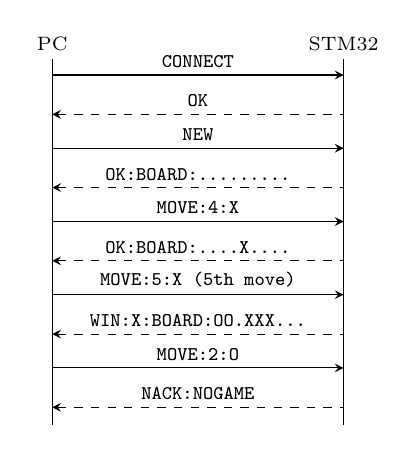
\begin{tikzpicture}[x=1cm,y=1cm]
 \node[font=\scriptsize] at (0,0.35) {PC};\node[font=\scriptsize] at (3.7,0.35) {STM32};
 \draw (0,0.15) -- (0,-4.5);\draw (3.7,0.15) -- (3.7,-4.5);
 \seqpair{-0.05}{CONNECT}{OK}
 \seqpair{-0.98}{NEW}{OK:BOARD:.........}
 \seqpair{-1.91}{MOVE:4:X}{OK:BOARD:....X....}
 \seqpair{-2.84}{MOVE:5:X (5th move)}{WIN:X:BOARD:OO.XXX...}
 \seqpair{-3.77}{MOVE:2:O}{NACK:NOGAME}
\end{tikzpicture}\\[2pt]{\footnotesize (a) X wins}
\end{minipage}\hfill
\begin{minipage}[t]{0.49\linewidth}\centering
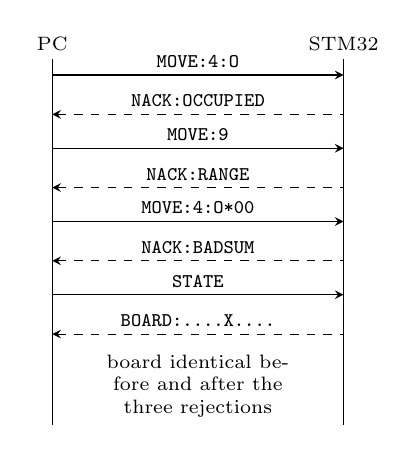
\begin{tikzpicture}[x=1cm,y=1cm]
 \node[font=\scriptsize] at (0,0.35) {PC};\node[font=\scriptsize] at (3.7,0.35) {STM32};
 \draw (0,0.15) -- (0,-4.5);\draw (3.7,0.15) -- (3.7,-4.5);
 \seqpair{-0.05}{MOVE:4:O}{NACK:OCCUPIED}
 \seqpair{-0.98}{MOVE:9}{NACK:RANGE}
 \seqpair{-1.91}{MOVE:4:O*00}{NACK:BADSUM}
 \seqpair{-2.84}{STATE}{BOARD:....X....}
 \node[font=\scriptsize,text width=3cm,align=center] at (1.85,-4.0) {board identical before and after the three rejections};
\end{tikzpicture}\\[2pt]{\footnotesize (b) rejections (board \code{....X....})}
\end{minipage}
